% Preamble
% ---
\documentclass[a4paper]{article}

% Packages
% ---
\usepackage{bm}
\usepackage[spanish,es-nodecimaldot]{babel}
\usepackage[utf8]{inputenc}
\usepackage[T1]{fontenc}
\usepackage{parskip}
\usepackage{fancyhdr}
\usepackage{mathtools}
\usepackage{amsmath}
\usepackage[htt]{hyphenat}
\usepackage{capt-of}
\usepackage{graphicx}
\graphicspath{ {./images/} }

% Pagestyles
% ---
\pagestyle{fancy}
\rhead{Roselló Beneitez, N. U.; Roselló Oviedo, M.}
\lhead{APR: Práctica sobre MLP}
\fancyfoot[C]{\thepage}

% Main
% ---
\begin{document}

\author{Roselló Beneitez, N. U.; Roselló Oviedo, M.}
\title{APR: Práctica sobre Redes Neuronales Multicapa (MLP)}
\date{6 de Enero de 2020}
\maketitle{}
\thispagestyle{empty}

\newpage
\tableofcontents
\listoffigures

\newpage
\section{Descripción de la práctica}
\quad En esta práctica se ha trabajado con redes neuronales multicapa en Octave mediante la librería \textit{nnet}, la cual dispone de sus propios métodos auxiliares con los que entrenar un \textit{multilayer perceptron}.

\quad La primera parte de la práctica, de carácter didáctico e iniciativo, consiste en experimentar con el corpus \textit{hart} para familiarizarse con la metodología de la librería, y no se haya incluida en esta memoria. La segunda parte, la cual desarrollaremos a continuación, se centra en la clasificación de dígitos de la base de datos MNIST.

\section{Redes neuronales en MNIST}
\quad 

\begin{center}
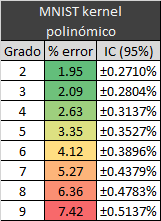
\includegraphics[width=100px]{2_mnist}
\captionof{figure}{asdf}
\end{center}

\section{Conclusiones}
\quad 

\end{document}
